\chapter{Myocardial Imaging and Echocardiography} \label{chap:strain}
\begin{comment}
[ ] Short about cardiology and echocardiography history
[ ] Short about the heart, and its anatomy
[ ] Even shorter about ultrasound, the different views, and what parts of the heart can be seen in them.
[ ] Method for extracting strain curves from ultrasound videos.
[ ] Explain the different diagnosises that will be encountered in this thesis.
[ ] Explain anatomical reasoning for why symptoms for certain diagnosis are evident in strain curves.
[ ] Summarize chapter
\end{comment}

This chapter will describe the basic structure of the heart muscle, give an introduction to ultrasound imaging and echocardiography, explain how longitudinal strain curves, and \acrfull{ef} is estimated and detail the causes of the heart diseases enountered in this work.

\section{Basic Cardiology}
\begin{comment}
[ ] Short about cardiology and echocardiography history
[ ] Short about the heart, and its anatomy
\end{comment}

The heart is an autonomous muscle that is responsible for pumping oxygenated blood from the lungs, into the rest of the body and pumping unoxegenated blood from the rest of the body, into the lungs. The heart can be divided into four separate chambers: The right atrium, the left atrium, the right ventricle and the left ventricle. The atriums are responsible for pumping unoxegenated blood into the lungs, and the ventricles are responsible for pumping oxygenated blood into the body. One heart cycle is the time period it takes the heart muscles to make a full contraction and relaxation. The period of the heart cycle where the heart relaxes, and fills with blood is called the \textit{diastole}, and the period of the heart cycle when the heart contracts and pumps blood throughout the body is called the \textit{systole}. Cardiology is the branch of medicine that deals with the heart, and parts of the vascular system \cite{cardiology_wikipedia}. Cardiologists are doctors that specialize in the field of cardiology. Echocardiography is a diagnostic tool used in cardiology to take images of muscle tissue in the heart, using ultrasound imaging. 

\section{Introduction to Ultrasound Imaging and Echocardiography}
\begin{comment}
[ ] Even shorter about ultrasound, the different views, and what parts of the heart can be seen in them.
\end{comment}

Ultrasound imaging is a diagnostic tool that is popular because it can give videos in real-time, it is relatively inexpenisve and has a lower associated health-risk compared to imaging alternatives \cite{medical_ultrasound_wikipedia}. In this section \textit{two dimensional B-mode ultrasound imaging} will be detailed, where the \textit{B} stands for \textit{brightness}. The frequency of the sound waves used in ultrasound imaging are in the range of 1 - 12 MHz, and the frequency chosen for wave pulses will decide the size of the objects that the method is able to resolute \cite{basic_ultrasound}. Ultrasound imaging works by emmitting pulses of ultrasound waves at myocardial tissue, the pulses are partially reflected by the different tissue structures, and are then sampled by a receiver upon return at the source that transmitted them, as illustrated in figure \ref{fig:us_reflect}.

\begin{figure}[H]
    \centering
    
\includegraphics[width=0.99\textwidth]{echocardiography/US_reflection.png}
    \caption{An illustration of how ultrsound pulses are partially reflected by many barriers of tissue. The horisontal arrows represent the pulses, where the relative sizes represent the amplitude of the pulse, and the vertical lines represent structures of tissue. The figure is inspired by figure 2 in \cite{basic_ultrasound}.}
    \label{fig:us_reflect}
\end{figure}

A sound waves will have different velocities depending of what medium it is travelling in. This ratio of velocities in the different mediums is what decides what amount of an incident wave is reflected when it hits a transition between two mediums. Since the velocity of the ultrasound waves in different mediums are known, and the time it takes for a transmitted pulse to return can be measured, one is able to calculate the distance to the tissue structure that reflected the transmitted pulse using equation \eqref{eq:dist}. 

\begin{equation}
    \mathrm{distance} = \frac{\mathrm{time}}{2 \times \mathrm{velocity}}
    \label{eq:dist}
\end{equation}

By plotting the intensity of the reflected pulses as a function of the distance to the point from which reflected it, one gets what is called a \textit{B-mode line}. Images created by two dimensional ultrasound imaging are polar plots of several B-mode lines that together make up a two dimensional intersectional image of a tissue structure. The procedure consists of emmitting a pulse, creating a B-mode line by the sampled reflections, rotating the transmitter, and repeating. This procedure is illustrated in figure \ref{fig:b_mode_search}.

\begin{figure}[H]
    \centering
    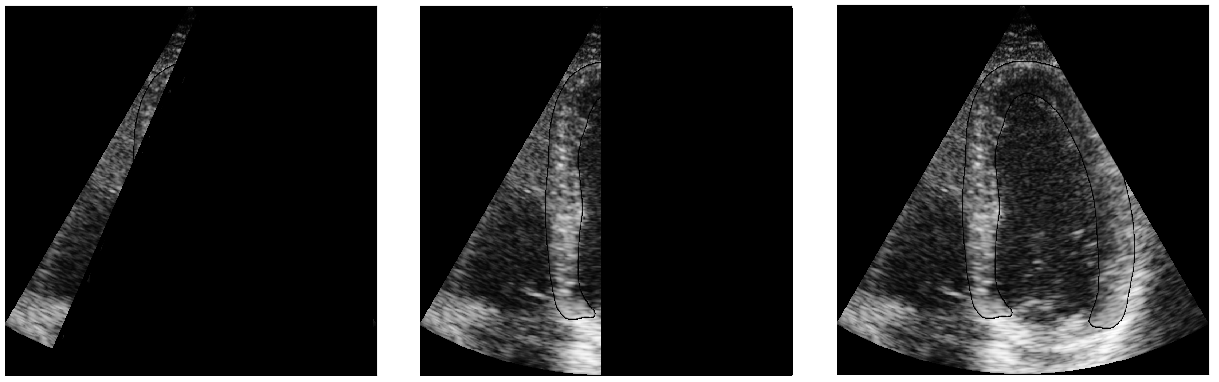
\includegraphics[width=0.99\textwidth]{echocardiography/b_mode_search.png}
    \caption{Illustration of how a two dimensional ultrasound image is put together by several individual B-mode lines. This figure is inspired by the graphipal illustrations in figure 7 in \cite{basic_ultrasound}.}
    \label{fig:b_mode_search}
\end{figure}

The specific method of echocardiography used to collect the data used in this thesis is called transthoracic echocardiography \cite{echocardiography_wikipedia}. In this method ultrasound images are produced by sending ultrasound waves through the ribs of a patient, from outside the body by locating the transmitter-reciever at the chest of the patient. The transthoracic echocardiography method is constricted by the ribs in as much that there are three intersectional images that can be extracted from the heart. These three intersections are referred to as \textit{views}, and there names are the \acrfull{4ch} view, \acrfull{2ch} view and the \acrfull{aplax} view, and examples of ultrasound images in all three views are given in figure \ref{fig:us_view_examples}.

\begin{figure}[H]
    \centering
    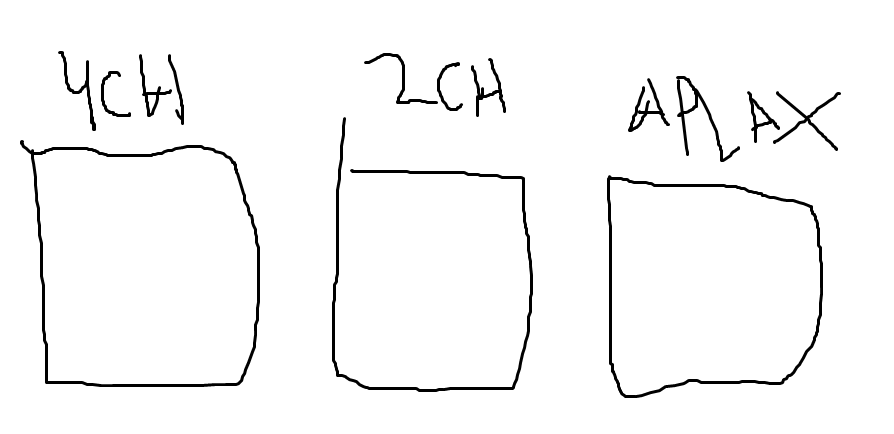
\includegraphics[width=0.99\textwidth]{echocardiography/us_view_examples.png}
    \caption{Examples of ultrasound images taken from the three views: \acrfull{4ch}, \acrfull{2ch} and \acrfull{aplax}. Note that these images are flipped vertically because the ultrasound images are taken from below the heart.}
    \label{fig:us_view_examples}
\end{figure}

It is commonplace among clinicians to focus on the state of health of the left ventricle of the heart, as it hold particularily much information about the state of health of the patient \cite{myocardial_imaging}. In clinical procedure the left ventricle is divided into 16, 17 or 18 segments. This work will follow the 18-segment model, as that is the model chosen by the clinician who has annotated the images. Figure \ref{fig:18_segment_model} shows how the left ventricle is divided into segments, and what the names of the individual segments are. When referring to the entire intersection of the left ventricle that is visible from a particular view, it is called the \textit{global segment}.

\begin{figure}[H]
    \centering
    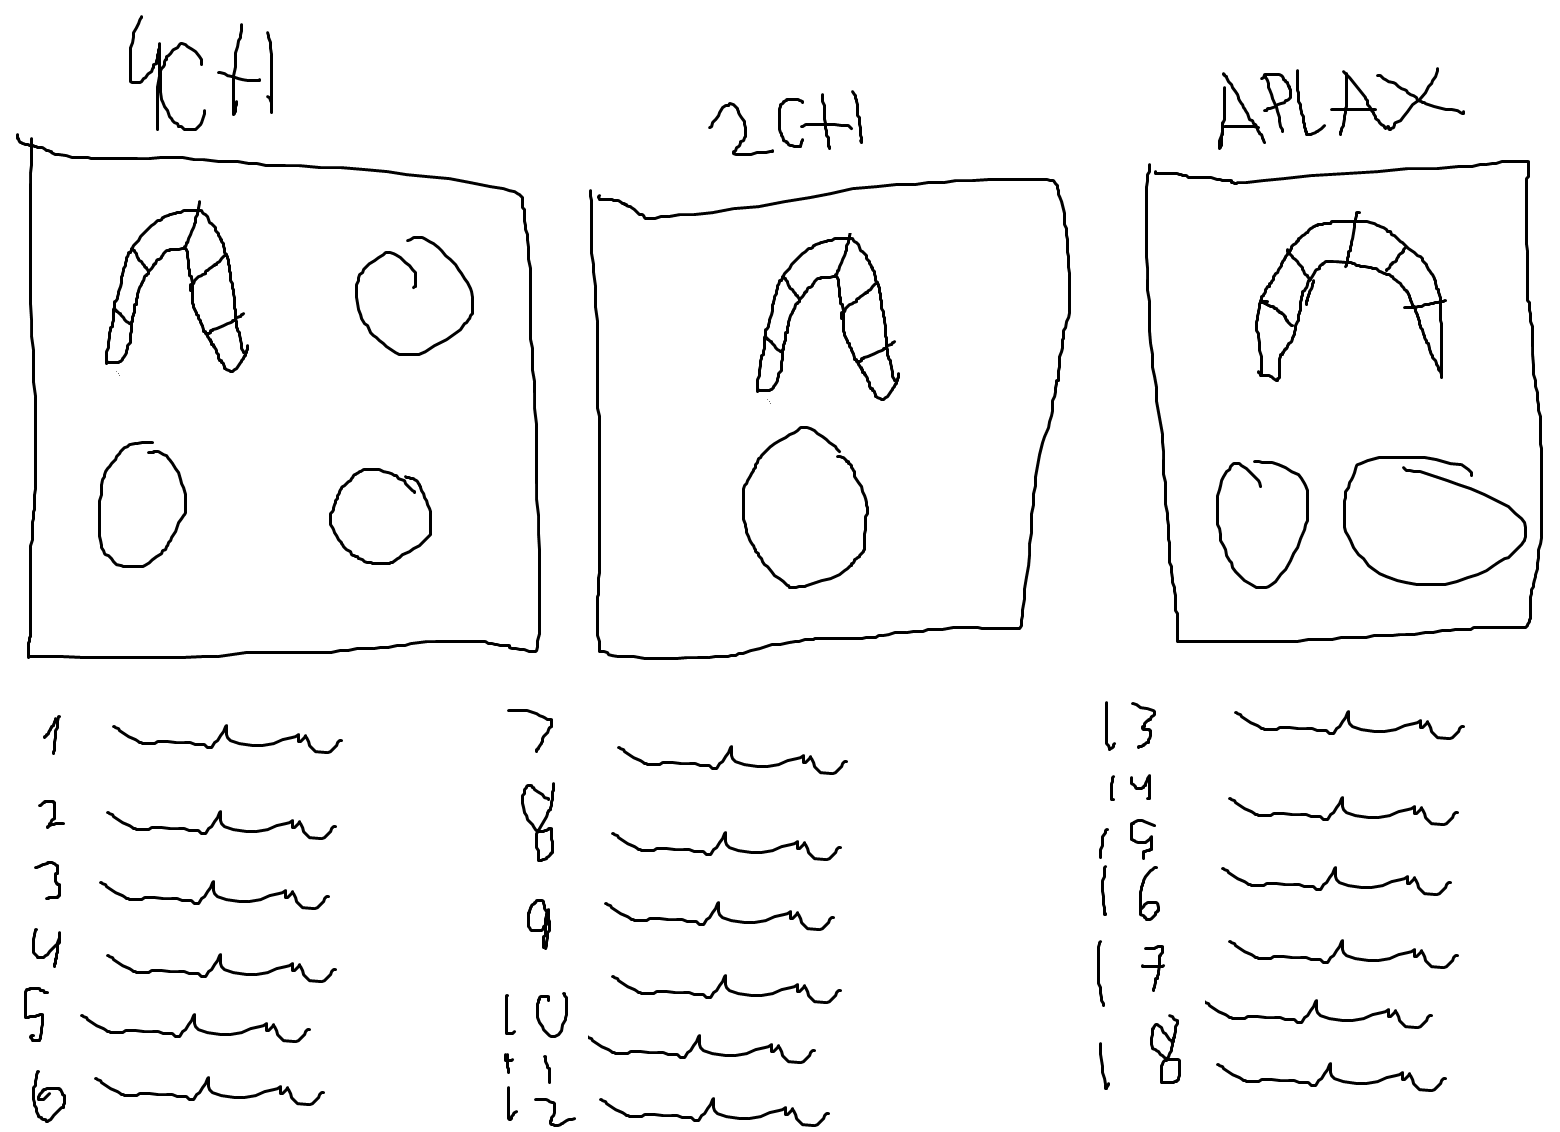
\includegraphics[width=0.99\textwidth]{echocardiography/18_segment_model.png}
    \caption{An illustration of the 18-segment model of the heart. It shows which segment can be seen in which view, and the names of the individual segments. Like in figure \ref{fig:us_view_examples} the images are flipped vertically, and so are the naming conventions. The names of the chambers are given from the patients point of view, e.g. the \textit{left ventricle} is on the \textit{left} from the patients point of view.}
    \label{fig:18_segment_model}
\end{figure}

\section{Myocardial Strain Estimation and Ejection Fracture}
\begin{comment}
[ ] Method for extracting strain curves from ultrasound videos.
[ ] Examples of GLS and RLS
[ ] Define the peak systolic strain used in this work
[ ] Define Ejection fracture
\end{comment}

Strain is a relative measure of deformation, so it has no unit, and is measured in percentages in this work. This work will be concerned with the strain of the myocardial tissue of the left ventricle of the heart muscle. To estimate the strain of a particular segment, one must first define the boundaries of all the segments. There are many ways of doing this, but the most accurate method is for a clinician to draw the segment boarders by hand. The clinician that annotated the dataset used in this work segmented the images using the commercial tool ECHOPAC which is developed by GE HealthCare\footnote{https://www.gehealthcare.com/products/ultrasound/vivid/echopac}. After the boundaries between the segments have been defined the centerline between the vertical boundaries is estimated, as illustrated by the BLUE line in figure \ref{fig:strain_estimation}. It is the length of the centerline which is used to estimate the strain curve of a segment during the period of one heart cycle. As strain is a relative measure, one needs to define a reference length from which the other strain values are calculated with regard to. This could be the length of the segment during the first frame, the length of the segment when it is at its longest, the length of the segment when it is at its shortest or the length of the segment in any other ultrasound image. Let the length of the segment in the reference image be denoted $L_r$, and let the length of the segment in image $t$ be denoted $L_t$. The strain value of a segment in image $t$, $s(t)$ is then given by equation \eqref{eq:strain}. The strain of a segment in the reference image will then be $0\%$, and the strain of the segment in the other images will be a percentage relative to the reference image. \bigskip

\begin{equation}
    s(t) = \frac{L_t - L_r}{L_r}
    \label{eq:strain}
\end{equation}

\begin{figure}[H]
    \centering
    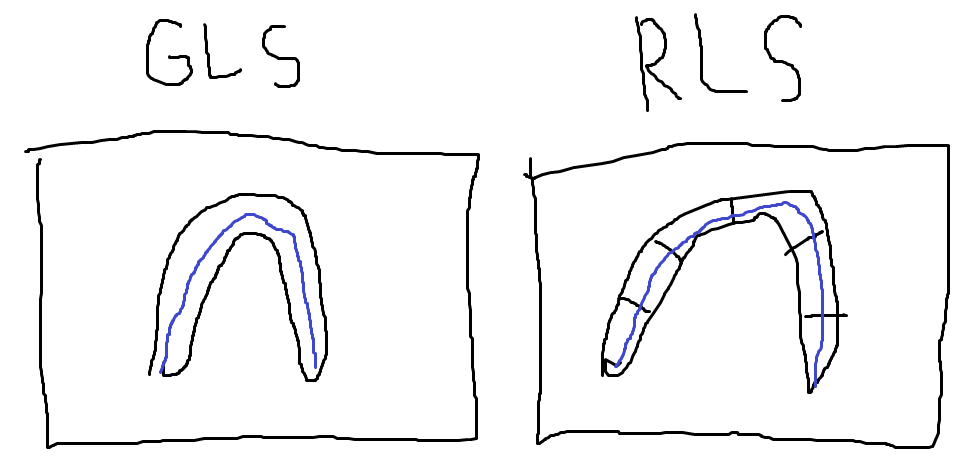
\includegraphics[width=0.99\textwidth]{echocardiography/strain_estimation.png}
    \caption{Illustration of how strain of a segment is estimated. Note that the segment borders drawn on these images are only illustrative, and are not the actual segment borders used to estimate the strain. (a) shows the strain estimation of the global segment, and (b) shows the strain estimation of the regional segments.}
    \label{fig:strain_estimation}
\end{figure}

By collecting all the strain values of a segment from the different ultrasound images into a time series, one gets a \textit{strain curve}. If the strain curve consists of strain values estimated from a global segment as depicted in figure \ref{fig:strain_estimation}a, the curve is called a \acrfull{gls} curve. If the strain values are estimated from one of the six regional segments, as depicted in figure \ref{fig:strain_estimation}b, the curves are called \acrfull{rls} curves. In diagnostic procedure it is common to extract specific values from the longitudinal strain curves. Typical strain values extracted are the peak value during the systole, the peak value during the diastole, trough values during the systole and trough values during the diastole. Figure \ref{fig:pss_illustration} shows what a typical longitudinal strain curve looks like, the peak and trough values are illustrated by red dots on the strain curve. The colour shading under the curves illustrate whether the heart cycle is in systole (blue), or diastole (red). In this work specific strain values will be tested as input data for classification models, the value that is extracted is the smallest strain value during the systole. This extracted strain value will be referred to as \textit{peak systolic strain}.

\begin{figure}[H]
    \centering
    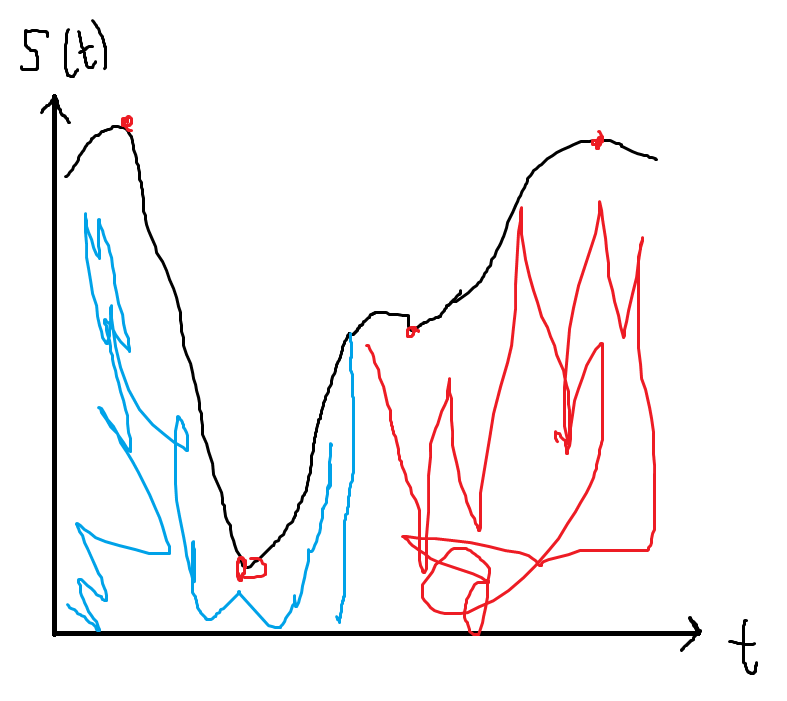
\includegraphics[width=0.99\textwidth]{echocardiography/pss_illustration.png}
    \caption{Example of a longitudinal strain curve. Red dots indicate peak and trough values, and the shading below the curves indicate whether the heart cycle is in systole (blue) or diastole (red).}
    \label{fig:pss_illustration}
\end{figure}

The \acrfull{ef} of the left ventricle is is a health parameter that is used to diagnose patients with heart failure \cite{myocardial_imaging}. Similar to segment strain \acrshort{ef} is a relative measure, it is the relative difference in volume of the left ventricle when it is fully relaxed, and when it is fully contracted. \acrshort{ef} is numerically computed using the two dimensional intersectinal images given by the three ultrasonic views provided by transthoracic echocardiography. \textcite{myocardial_imaging} state that \acrshort{ef} values below $45\%$ are regarded as abnormal, and should warrant further inspection of a patient with regard to the possibility of contracting heart failure.

\section{Heart Diseases}
\begin{comment}
[ ] Explain the different diagnosises that will be encountered in this thesis.
[ ] Explain anatomical reasoning for why symptoms for certain diagnosis are evident in strain curves.
\end{comment}

Heart failure is the term used to describe when the heart muscle is unable to pump sufficient volumes of blood to the other muscles and organs in the body \cite{medicine_net}. So in a sense, heart failure can be considered as a degree of severity rather than a diagnosis. The heart diseases that are encountered in this work will mostly fall within the category of \textit{myocardial infarction}, which is also known as \textit{heart attack}. Myocardial infarction is encountered in two varieties \acrfull{stemi} and \acrfull{nstemi}. \acrshort{stemi} gets its name from the elevation of the ST segment of an electrocardiogram of a patient, which is a test performed on patients experiencing myocardial infarction \cite{ecg_stemi}. \acrshort{nstemi} then gets its name from the fact that the ST segment is not elevated in an electrocardiogram. \acrshort{stemi} is associated with a full blockage in one of the arteries supplying the heart with blood, and \acrshort{nstemi} is often associated with a partial blockage in one or several coronary arteries \cite{ambulanseforum}. Therefore, in many cases the \acrshort{nstemi} diagnosis does not require the same acute medical treatment that the \acrshort{stemi} diagnosis does. The heart diseases encountered that do not fall within the \acrshort{stemi} or \acrshort{nstemi} categories, were not given a specific label and are hence labelled as OTHER. \bigskip

One of the issues with using low \acrshort{ef} values to diagnose heart failure alone is that there is a significant subgroup that does not show low \acrshort{ef} values. Some patients that have heart diseases experience a growth in the muscle tissue around the heart, this is called \textit{hypertrophy}. The additional muscle reduces the absolute volume of the left ventricle. A reduced range of contraction will not be visible in the \acrshort{ef}, because the volume of the relaxed heart muscle is also reduced. When heart failure occurs, without being evident in the \acrshort{ef} values it is referred to as \textit{heart failure with preserved ejection fraction}. \bigskip

Reduced blood supply to parts of the heart muscle is also visible in ultrasound images, specifically in the range of motion of the specific regional segments. The reduction in blood supply will over time damage the myocardial tissue of the segment, this is evident by the reduced range of motion of the segment. Different segments are given \textit{segment indications} based on how good the ''quality'' of the range of motion of a segment is. The different labels of interest are \textit{normal}, if the range of motion of a segment looks normal, \textit{hyperkinetic} if the range of motion is increased and \textit{hypokinetic}, \textit{dyskinetic} and \textit{akinetic} are labels used for segments that show reduced ranges of motion. Section \ref{sec:target} will explore whether these attributes can be seen in the \acrshort{rls} curves.

\section{Chapter Summary}

In this chapter the basic structure of the heart muscle is detailed, the technology behind ultrasound imaging and echocardiography is introduced, the estimation of longitudinal strain curves, and \acrshort{ef} is explained and the heart diseases enountered in this work are expanded upon. The heart is made up of two atriums that are responsible for pumping unoxegenated blood into the lungs, and two ventricles that pump oxygenated blood from the lungs into the rest of the body. B-mode ultrasound images are made by transmitting pulses of ultrasound waves, which are reflected by myocardial tissue and are sampled at the reciever. transthoracic echocardiography is a method of echocardiography used to obtain ultrasound images of the heart. It is performed by placing the transmitter/reciever at the ribs of a patient, and provides three intersectional images of the heart \acrshort{4ch}, \acrshort{2ch} and \acrshort{aplax}. Strain of the different segments of the left ventricle is estimated by drawing the boundaries of the segments using ECHOPAC, and calculating strain using equation \eqref{eq:strain}. \acrshort{ef} is the measure of relative difference in volume of a fully relaxed left ventricle heart mucle, and a fully contracted one. The most common heart diseases encountered in this work are \acrshort{stemi}, and \acrshort{nstemi}, any other diseases were not labelled in the dataset, and will hence be labelled as OTHER. Restricted blood supply to specific segments becomes evident in the ultrasound images, specifically in the range of motion of the individual segments. individual segments are given \textit{segment indication} labels describing the quality of their range of motion. 